\section{Beobachter zur Ermittlung von $\varphi$}
In dem letzten Abschnitt sind die Nachteile des Komplementärfilters aufgezeigt worden. Aus diesem Grund wird am Beispiel des auf einer Kante balancierenden Würfels ein Luenberger-Beobachter entworfen, um den Winkel $\varphi$ zu bestimmen. Hierfür wird wieder das System
\begin{equation}
\textfrak{D} \equiv \left\{ \begin{array}{ll}
\bs{x}(k+1) &= \bs{A}\cdot \bs{x}(k) + \bs{b}\cdot u(k)
\\
\bs{y}(k) &= \underbrace{\begin{bmatrix}
\bs{0}^{2\times 1} & \bs{I}^{2\times 2}
\end{bmatrix}}_{= \bs{C}} \cdot \bs{x}(k)
\end{array}\right.\,, \hspace{35pt} \bs{x}=\begin{bmatrix}
\varphi \\ u_K \\ u_R
\end{bmatrix}
\label{eq_edge_system}
\end{equation}
betrachtet, wobei lediglich die Zustandsgrößen $u_K$ und $u_R$ messbar seine. Aus dem Kalmankriterium ergibt sich, dass das System vollständig beobachtbar ist. D.h. der Verlauf der Zustandsgrößen kann aus dem Ausgangsvektor und der Eingangsgröße rekonstruiert werden. Hierfür wird ein Luenberger-Beobachter verwendet. Das Grundprinzip des Beobachters besteht darin einen Schätzwert $\bs{\hat{x}}$ aus dem Modell (\ref{eq_edge_system}) zu berechnen. Bei diesem Ansatz führt bereits eine minimale Abweichung zwischen dem Modell und dem realen System zu einem kontinuierlich zunehmenden Schätzfehler. Um diesen Fehler zu eliminieren wird das in der Regelungstechnik bewährte Konzept der Fehlerrückführung verwendet. Da der Zustandsvektor nicht messbar ist wird  die Differenz $\Delta \bs{y}$ der Ausgangsvektoren über die so genannte Beobachtermatrix $\bs{L}$ zurückgeführt.
\begin{figure}[h!]
\centering
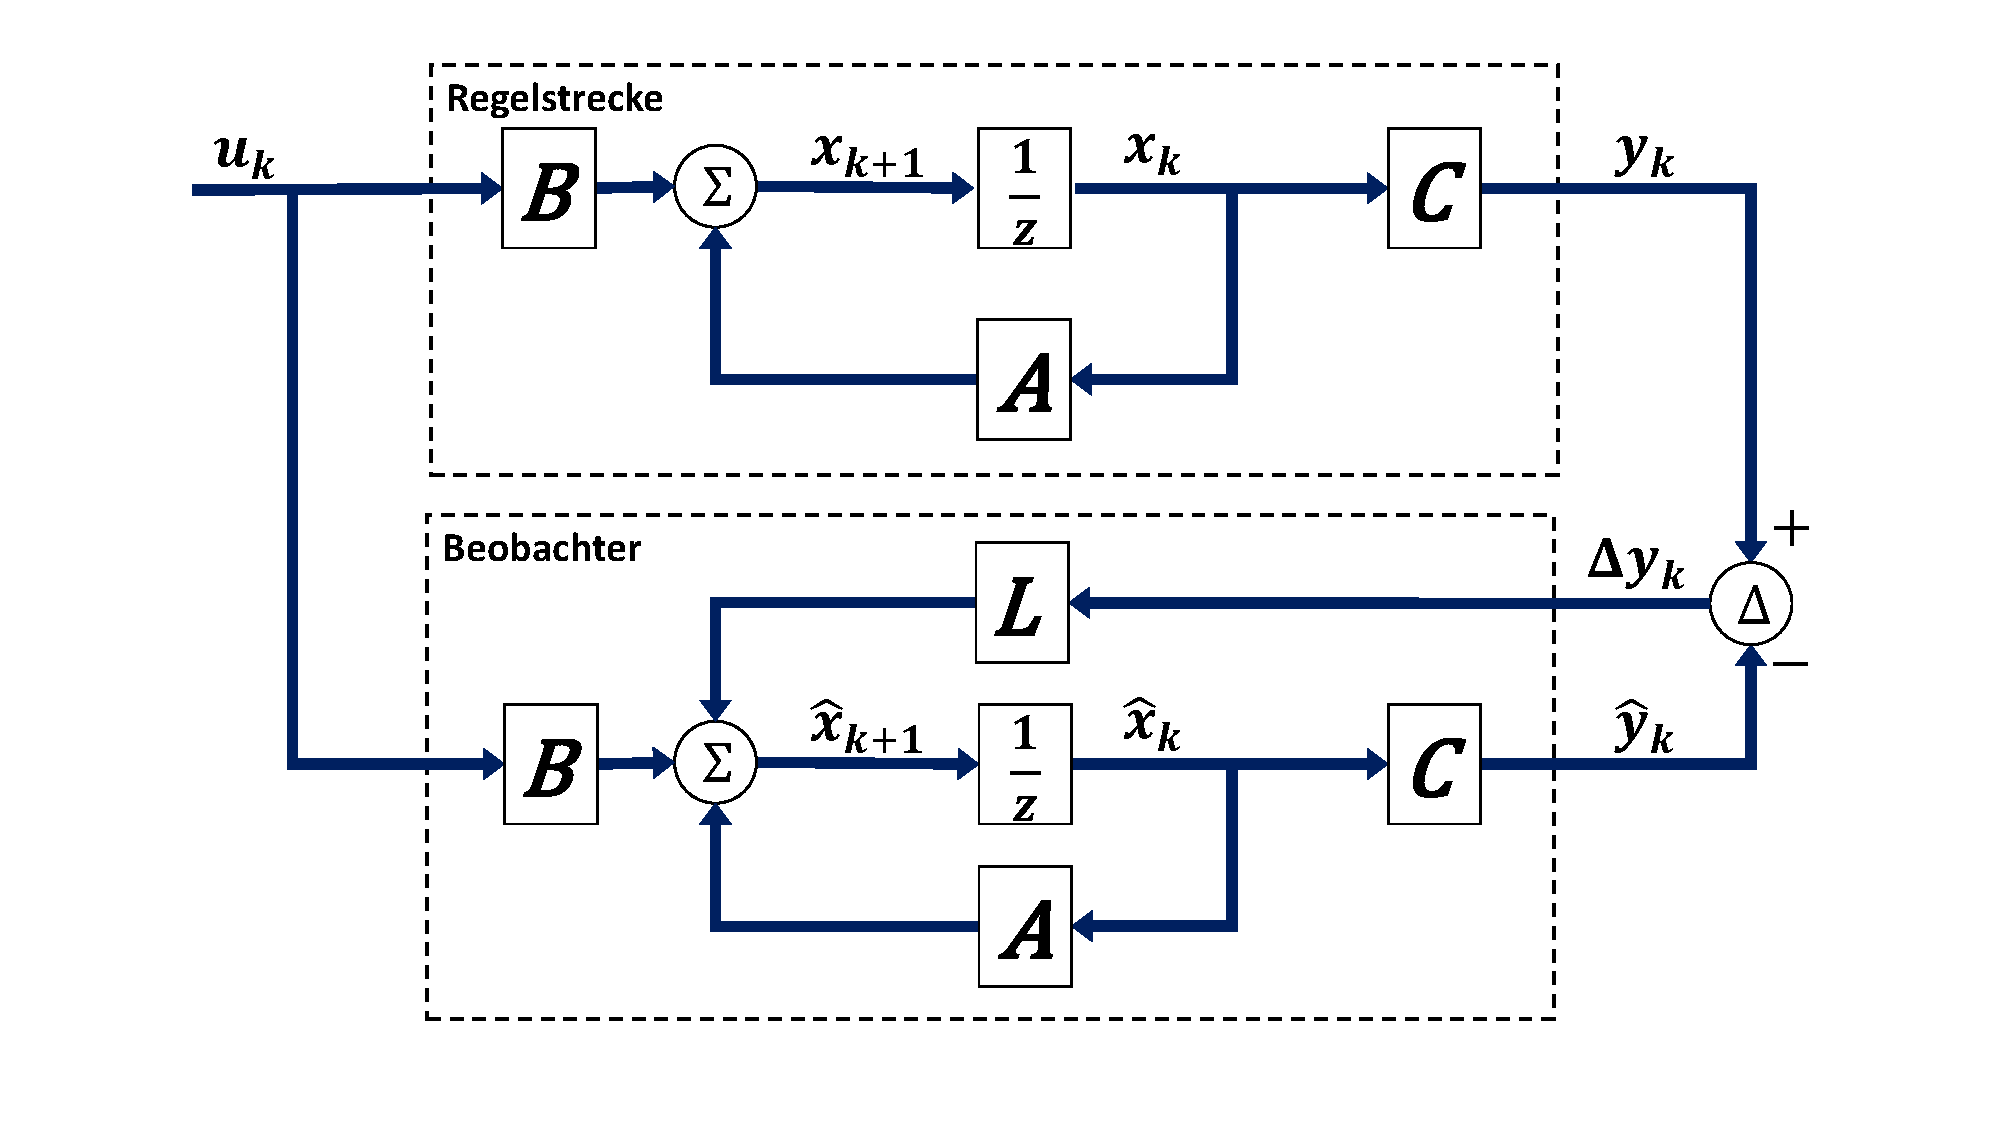
\includegraphics[width=1\linewidth, trim={1cm 1cm 1cm 1cm}, clip]{img/Observer}
\caption{Blockschaltbild des Luenberger-Beobachters}
\end{figure}

Um das Verhalten des Beobachters zu untersuchen wird der Schätzfehler $\bs{e}(k) = \bs{x}(k) - \bs{\hat{x}}(k)$ betrachtet.
\begin{equation}
\begin{split}
\bs{e}(k+1) &= \bs{x}(k+1) - \bs{\hat{x}}(k+1) \\
&= [\bs{A}\cdot \bs{x}(k) + \bs{B}\cdot \bs{u}(k)] - [\bs{A}\cdot \bs{\hat{x}}(k) + \bs{B}\cdot \bs{u}(k) +\bs{L}\bs{\hat{y}}(k)]
\\
&= [\bs{A}\cdot (\bs{x}(k) - \bs{\hat{x}}(k))] - \bs{L}\bs{C}\cdot[\bs{x}(k)-\bs{\hat{x}}(k)] 
\\
&= \bs{A}\cdot \bs{e}(k) - \bs{LC}\cdot\bs{e}(k) = (\bs{A}-\bs{LC})\cdot \bs{e}(k)
\end{split}
\end{equation}
Hieraus folgt, dass der Verlauf des Schätzfehlers $\bs{e}(k)$ ein geschlossenen System darstellt. Wird die Beobachtermatrix $\bs{L}$ so gewählt, dass die Eigenwerte der Systemmatrix $\bs{A}-\bs{LC}$ im Einheitskreis liegen konvergiert der Schätzfehler gegen null. Da die Eigenwerte durch die Transponierung einer Matrix nicht verändert werden, kann die Entwurfsaufgabe als
\begin{equation}
\left\vert \lambda_i\left\{\bs{A}^T-\bs{C}^T\bs{L}^T\right\}\right\vert \overset{!}< 1
\end{equation}
formuliert werden. Diese Problemstellung entspricht der Entwurfsaufgabe eines gewöhnlichen Zustandsreglers, weshalb die bereits vorgestellten Verfahren für den Reglerentwurf auch für die Bestimmung der Beobachtermatrix $\bs{L}$ verwendet werden können. Für diesen Anwendungsfall wird der Beobachter optimal im Sinne des quadratischen Gütekriteriums entworfen. Als Gewichtungsmatrix $\bs{R}$ wird die Kovarianzmatrix des Ausgangvektors $\bs{y}$ verwendet. Die Matrix $\bs{Q}$ wird empirisch ermittelt. Prinzipiell unterliegt der Beobachter keiner Stellgrößenbeschränkung, da die Rückführung von $\Delta\bs{y}$ digital berechnet wird. Allerdings wirkt ein Messrauschen proportional zu $\bs{L}$ auf den Schätzwert $\bs{\hat{x}}$ ein. Aus diesem Grund werden die Elemente der Gewichtungsmatrix $\bs{Q}$ möglichst klein gewählt. Die folgenden Abbildung zeigen den Verlauf des System, wobei der Regler mit Hilfe des geschätzten Zustandvektors $\bs{\hat{x}}$ berechnet wird. Die folgende Abbildung zeigt den Verlauf der Zustandsgrößen und der Stellgröße im geschlossenen Regelkreis, wobei der Regler mittels des geschätzten Zustandvektors $\bs{\hat{x}}$ berechnet wurde.
\begin{figure}[H]
\centering
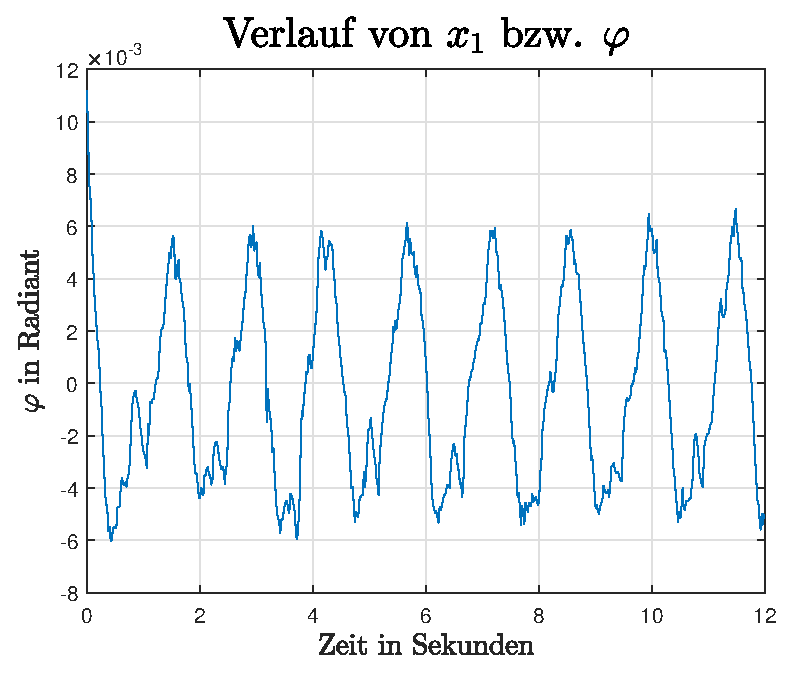
\includegraphics[width=0.43\linewidth]{img/edge_exp3_phi.eps}
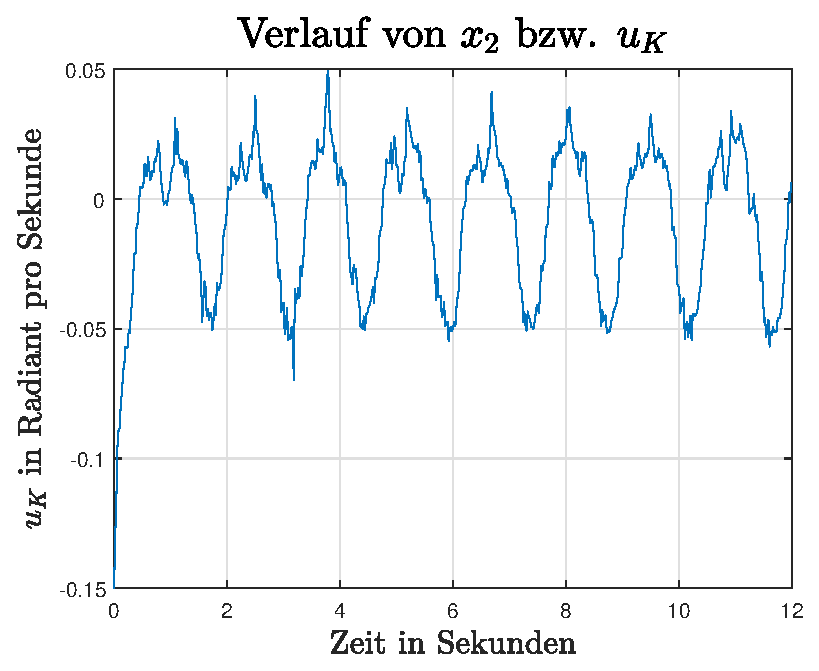
\includegraphics[width=0.43\linewidth]{img/edge_exp3_uk.eps}
\vspace{0.5cm}

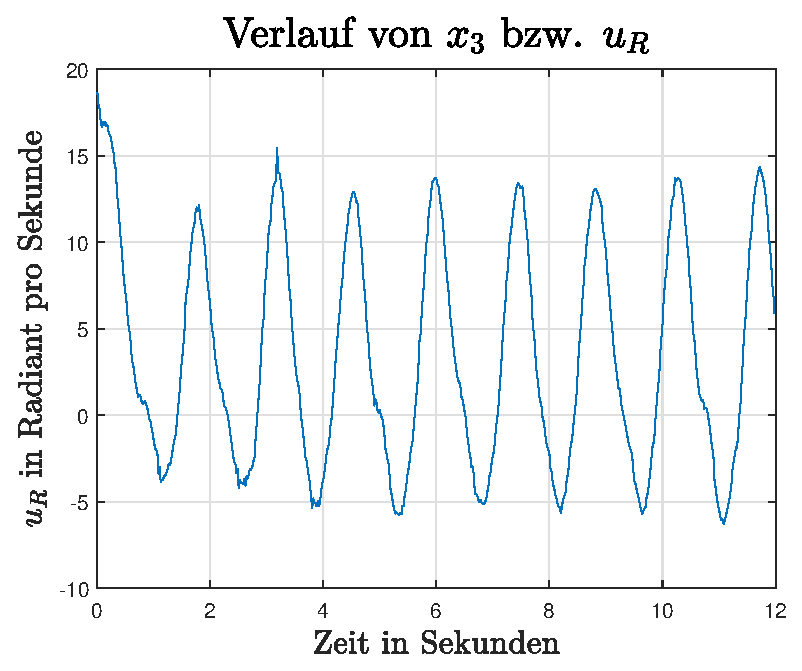
\includegraphics[width=0.43\linewidth]{img/edge_exp3_ur.eps}
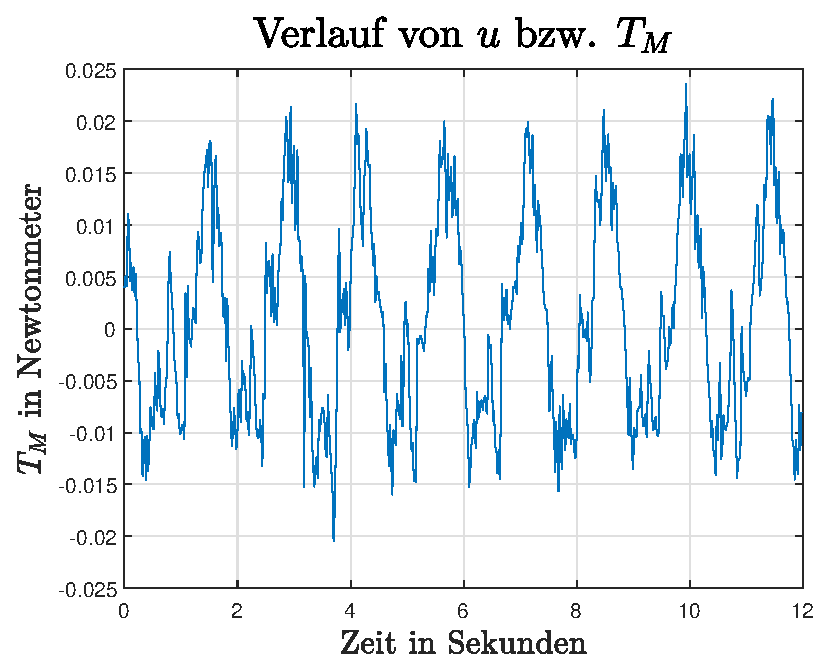
\includegraphics[width=0.43\linewidth]{img/edge_exp3_tm.eps}
\label{plots_phiobs}
\caption{Verlauf des geschätzten Zustandvektors und der Stellgröße}
\end{figure}

Der Versuch zeigt, dass das System mit dem Beobachter lediglich grenzstabil ist und mit einer konstanten Amplitude oszilliert. Eine mögliche Begründung für dieses Verhalten ist die Wahl der Beobachtermatrix. Um den Einfluss des Messrauschens zu minimieren wurde die Gewichtungsmatrix $\bs{Q}$ so gewählt, dass eine Beobachtermatrix mit relativ kleinen Elementen resultiert. Hieraus folgt, dass die Eigenwerte des Beobachters nahe an dem Einheitskreis liegen und somit bereits kleine Ungenauigkeiten in den Modellparametern genügen um grenzstabile Eigenwerte zu erhalten. Werden die Eigenwerte des Beobachters näher zu dem Urpsrung gerückt wird der Beobachter allerdings instabil, da das Messrauschen den Schätzwert $\bs{\hat{x}}$ zu stark beeinflusst. Dieses Problem ist darauf zurückzuführen, dass der Luenberger-Beobachter für ein deterministisches System entworfen wird und die stochastischen Störung lediglich indirekt bei dem Entwurfsverfahren berücksichtigt werden. Eine Lösung für dieses Problem stellt das Kalman-Filter dar, welches für die Beobachtung von linearen, zeitvarianten und stochastisch gestörten Systemen genutzt werden kann. Des weiteren bestehen Erweiterung wie das Extended-Kalman-Filter um das Konzept auf nichtlineare Systeme zu übertragen. 
Die Vorteile dieses Ansatz bestehen einerseits darin, dass mit einer Erweiterung auf nichtlineare Systeme ein global gültiges Schätzverfahren entsteht. Andererseits wird durch die Schätzung der Winkel $\varphi_i$ die Anzahl der benötigten Sensoren reduziert. Ebenso kann ein Kalman-Filter genutzt werden um die verrauschten Beschleunigungsmessungen mit den Winkelgeschwindigkeiten zu fusionieren. Im ersten Schritt ist allerdings eine Systemidentifikation und Parameterschätzverfahren durchzuführen, da eine mögliche Ursache für die verbleibende Schwingungen eine geringe Modellgüte ist. Derartige Fehler wirken sich ebenso negativ auf ein Kalman-Filter aus.